\section{Relationen}

\begin{frame}
	\frametitle{Kartesisches Produkt}
	\begin{block}{Definition}
		Das \textbf{kartesische Produkt} zwischen zwei Mengen $M$ und $N$ ist definiert als
		$$M \times N = \{ (m,n) \mid m \in M, n \in N \}$$
		Induktiv definiert man das kartesische Produkt beliebig vieler Mengen (VL).\\
		Es enthält n-Tupel der Form $(m_1, m_2, ..., m_n)$.
	\end{block}

	\pause
	\begin{block}{Beispiel}
		$\{a,b\} \times \{1, 2, 3\} = \{(a, 1), (a, 2), (a, 3), (b, 1), (b, 2), (b, 3)\}$ \\
		$\{0, 1\}^3 = \{(0, 0, 0), (0, 0, 1), (0, 1, 0), (0, 1, 1), (1, 0, 0), (1, 0, 1), (1, 1, 0), (1, 1, 1)\} $ \\[0.5em]
		Für jede Menge $M$ gilt: $ M \times \emptyset = \pause \emptyset $
	\end{block}
\end{frame}

\begin{frame}
	\frametitle{Relationen}
	\begin{block}{Definition}
		Sind $A$ und $B$ zwei Mengen, so beschreibt eine Relation $R$ eine Teilmenge der Paare $(a,b) \text{ mit } a \in A, b \in B$.
		$$R \subseteq A \times B$$ Meist ist diese Relationszugehörigkeit implizit durch eine Vorschrift gegeben. \\
		Zwei Elemente $a \in A$, $b \in B$ stehen in der Relation R zueinander, wenn $(a, b) \in R$.
	\end{block}
	
	\pause
	\begin{block}{Beispiel}
		Betrachten wir die Relation $ \leq \text{auf} \; \nN_0 \times \nN_0 $. \\
		Dann gilt $ \leq \; = \{(m, n) \mid m \leq n \} = \{(0, 0), (0, 1), (1, 1), (0, 2), ...\} $
	\end{block}
\end{frame}

\begin{frame}
	\frametitle{Relationen}	
	\begin{block}{Beispiel}
		$ P = \nZ \times \nN_+ \times \nN_0 $ \\
		$ \cdot \; = \{(n, m, r) \in P \mid n * m = r \} \subseteq P $ \\[0.5em]
		\pause
		$ \cdot \; = \{(0, 1, 0), (0, 2, 0), (1, 1, 1), (1, 2, 2), (6, 7, 42) ...\} $ \\[0.5em]
		$ (-1, 1, -1), (42, 0, 0) \notin \cdot $\\[1em]
		\pause
		Immer auf die Grundmenge achten!
	\end{block}
\end{frame}

\begin{frame}
	\frametitle{Eigenschaften von Relationen}
	\begin{block}{Totalität}
		Eine Relation $R \subseteq A \times B$ heißt linkstotal, wenn es für jedes Element $a \in A$ ein zugehöriges Element $b \in B$ gibt, mit $$(a,b) \in R$$ Für rechtstotal gilt die analoge Aussage.
	\end{block}
	
	\pause
	\begin{block}{Eindeutigkeit}
		Eine Relation $R \subseteq A \times B$ heißt linkseindeutig, wenn für jedes Element $b \in B$ und $a_1, a_2 \in A$ mit $$(a_1,b) \in R \text{ und } (a_2,b) \in R$$ gilt $a_1 = a_2$. \\
		Für rechtseindeutig gilt die analoge Aussage.
	\end{block}
\end{frame}

\subsection{Aufgabe 1}
\begin{frame}
	\frametitle{Aufgabe (WS 2010) Teil 1}
	Es sei $A$ die Menge aller Kinobesucher in einer Vorstellung und $B$ die Menge aller Sitzplätze. Die Relation $R$ ordnet den Kinobesuchern die Sitzplätze zu:
	$$ R \subseteq A \times B$$
	\begin{itemize}
		\item Was bedeutet es im Kino, wenn $R$ linkstotal, linkseindeutig, rechtstotal, rechtseindeutig ist?
	\end{itemize}
\end{frame}

\begin{frame}
	\frametitle{Lösung}
	\textit{Was bedeutet es im Kino, wenn $R$ linkstotal, linkseindeutig, rechtstotal, rechtseindeutig ist?} \\[2em] \pause
	\emph{linkstotal}: jedem Kinobesucher wird mindestens ein Sitzplatz zugeteilt \\ \pause
	\emph{linkseindeutig}: jeder Sitzplatz ist von höchstens einem Kinobesucher belegt \\ \pause
	\emph{rechtstotal}: jeder Sitzplatz ist von mindestens einem Kinobesucher belegt \\ \pause
	\emph{rechtseindeutig}: kein Kinobesucher belegt mehr als einen Sitzplatz \\
\end{frame}

\begin{frame}
	\frametitle{Funktionen}
	\begin{block}{Definition}
		Ist eine Relation $f \subseteq A \times B$ rechtseindeutig und linkstotal, so nennt man sie \textbf{Funktion} oder \textbf{Abbildung} mit \textbf{Wertebereich} $A$ und \textbf{Zielbereich} $B$.\\[1em]
		Man schreibt 
		\begin{align*}
			f : A &\to B \\
			a &\mapsto b \text{ oder } f(a) = b
		\end{align*}
	\end{block}

	\pause
	\begin{block}{Wichtig}
		Funktionen immer \textbf{vollständig} angeben, also Definitionsbereich, Zielbereich sowie Abbildungsvorschrift. \\
		Auf die unterschiedlichen Pfeile achten (zwischen Definitions- und Zielbereich kein Strich am Ende des Pfeils)!
	\end{block}
\end{frame}

\begin{frame}
	\frametitle{Funktionen}
	
	\begin{block}{Definition}
		Eine linkseindeutige Funktion nennt man \textbf{injektiv}. \\
		Eine rechtstotale Funktion nennt man \textbf{surjektiv}. \\
		Erfüllt eine Funktion beide Eigenschaften, so nennt man sie \textbf{bijektiv}.
	\end{block}

	\begin{block}{Beispiel}
		\begin{align*}
			g : \{1, 2\} &\to \{3, 4\} \\
			1 &\mapsto 3 \\
			2 &\mapsto 4
		\end{align*}
		Wir haben explizit eine vollständige Abbildungsvorschrift angegeben.\\
		Als Relation geschrieben gilt $g = \{(1, 3), (2, 4)\}$, und $g$ ist bijektiv.
	\end{block}

\end{frame}

\begin{frame}
	\frametitle{Aufgabe (WS 2010) Teil 2}
	Es sei $A$ die Menge aller Kinobesucher in einer Vorstellung und $B$ die Menge aller Sitzplätze. Die Abbildung $f$ ordnet den Kinobesuchern die Sitzplätze zu:
	$$ f : A \to B$$
	\begin{itemize}
		\item Was wünschen sich die Kinobesucher: Eine injektive, surjektive oder bijektive Abbildung auf die Sitzplätze? Was wünscht sich der Kinobesitzer?
		\item In dieser Teilaufgabe nehmen wir an, 6 Kinobesucher besuchten ein Kino mit 8 Plätzen. Zeichnen Sie eine injektive Abbildung f.\\
		%Wie viele injektive Abbildungen gibt es?
	\end{itemize}
	
\end{frame}

\begin{frame}
	\frametitle{Lösung}
	\textit{Was wünschen sich die Kinobesucher: Eine injektive, surjektive oder bijektive Abbildung auf die Sitzplätze? Was wünscht sich der Kinobesitzer?} \\[2em] \pause
	Da $f$ eine Abbildung sein soll, muss sie linkstotal (jeder Besucher bekommt einen Platz) und rechtseindeutig (kein Besucher bekommt mehr als einen Platz) sein.\\
	\pause
	Ein Kinobesucher möchte alleine auf seinen Platz sein. Also wünscht er sich eine injektive (linkseindeutige) Funktion.\\ 
	\pause 
	Der Kinobesitzer möchte, dass das Kino voll ist und jeder Sitzplatz belegt. Er wünscht sich also eine surjektive (rechtstotale) Funktion.
\end{frame}

\begin{frame}
	\frametitle{Lösung}
	\textit{In dieser Teilaufgabe nehmen wir an, 6 Kinobesucher besuchten ein Kino mit 8 Plätzen. Zeichnen Sie eine injektive Abbildung f.} \\[2em] \pause
	
	\begin{figure}[H]
		\centering
		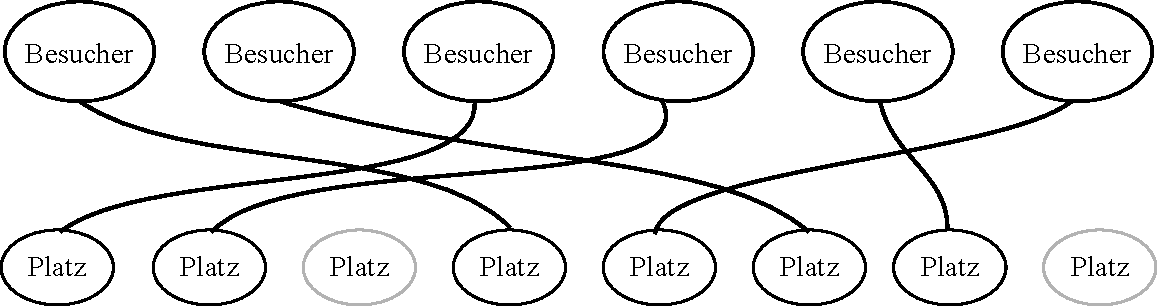
\includegraphics[scale=0.5]{Kinoabbildungen.pdf}
	\end{figure}
\end{frame}

%\begin{frame}
%	\frametitle{Lösung}
%	\textit{In dieser Teilaufgabe nehmen wir an, 6 Kinobesucher besuchten ein Kino mit 8 Plätzen. Wie viele injektive Abbildungen gibt es?} \\[2em] \pause
%	
%	Es gibt insgesamt $$8 \cdot 7 \cdot 6 \cdot 5 \cdot 4 \cdot 3 = 20160$$ injektive Abbildungen. \\[1em]
%	Der erste Besucher hat 8 Plätze zur Auswahl. Da aufgrund der Injektivität der nächste Besucher einen anderen Sitzplatz wählen muss, stehen ihm noch 7 Plätze zur Auswahl. Dies kann man für die restlichen Besucher fortsetzen.
%	
%\end{frame}

\subsection{Aufgabe 2}
\begin{frame}
	\frametitle{Aufgabe 2}
	
	Was kann man über die Surjektivität, Injektivität, Bijektivität folgender Abbildungen sagen? Begründen Sie jeweils kurz.
	
	\begin{alist}
		\item $f: \nR \to \nR: x \mapsto x^2$
		\item $f: \nR_+ \to \nR_+: x \mapsto x^2$
		\item $f: \nN_0 \to \nN_0 : x \mapsto \begin{cases} 42 &\text{wenn $x = 0$} \\ x - 1 &\text{sonst} \end{cases}$
	\end{alist}
\end{frame}

\begin{frame}
	\frametitle{Lösung}
	\begin{alist}
		\item $f: \nR \to \nR: x \mapsto x^2$ \\
		\pause
		Diese Funktion ist weder injektiv ($f(-2) = f(2) = 4$) noch surjektiv (Es gibt kein $x$ welches z.B. auf $-1 \in \nR$ abgebildet wird). Somit auch nicht bijektiv.
		
		\item $f: \nR_+ \to \nR_+: x \mapsto x^2$ \\
		\pause
		Wir können zu jedem $y \in \nR_+$ ein $x \in \nR_+$ angeben, so dass $f(x) = y$: $ x = \sqrt{y}$. \\
		Die Funktion ist also surjektiv, und da dieses x eindeutig ist auch injektiv. Also ist die Funktion bijektiv.
		
		\item $f: \nN_0 \to \nN_0 : x \mapsto \begin{cases} 42 &\text{wenn $x = 0$} \\ x - 1 &\text{sonst} \end{cases}$ \\
		\pause
		Diese Funktion ist nicht injektiv ($f(0) = f(43) = 42$), aber surjektiv (Für jedes $x \in \nN_0$ gilt: $x + 1 \in \nN_0 \text{ und } f(x+1) = x$). Somit nicht bijektiv.
	\end{alist}
\end{frame}

\begin{frame}
	\begin{block}{Wahr oder Falsch?}
		Sei $M$ eine beliebige endliche Menge und $f$ eine Abbildung $f : M \to M$.
		\begin{itemize}
			\truefalseQ{1}{myGreen}{Wenn $f$ injektiv ist, dann ist $f$ auch surjektiv.}{W}
			\truefalseQ{1}{myGreen}{Wenn $f$ surjektiv ist, dann ist $f$ auch injektiv}{W}
			\truefalseQ{4}{myRed}{Die beiden Aussagen gelten auch, wenn $M$ nicht endlich ist.}{F}
		\end{itemize}
	\end{block}

	\pause[5]
	\begin{block}{Gegenbeispiel im Unendlichen}
		$f : \nN_0 \to \nN_0, n \mapsto 2 * n $\\ 
		$g : \nN_0 \to \nN_0: n \mapsto \lfloor n/2 \rfloor$
	\end{block}
	
\end{frame}